% Options for packages loaded elsewhere
\PassOptionsToPackage{unicode}{hyperref}
\PassOptionsToPackage{hyphens}{url}
\PassOptionsToPackage{dvipsnames,svgnames,x11names}{xcolor}
%
\documentclass[
  ignorenonframetext,
]{beamer}
\usepackage{pgfpages}
\setbeamertemplate{caption}[numbered]
\setbeamertemplate{caption label separator}{: }
\setbeamercolor{caption name}{fg=normal text.fg}
\beamertemplatenavigationsymbolsempty
% Prevent slide breaks in the middle of a paragraph
\widowpenalties 1 10000
\raggedbottom
\setbeamertemplate{part page}{
  \centering
  \begin{beamercolorbox}[sep=16pt,center]{part title}
    \usebeamerfont{part title}\insertpart\par
  \end{beamercolorbox}
}
\setbeamertemplate{section page}{
  \centering
  \begin{beamercolorbox}[sep=12pt,center]{part title}
    \usebeamerfont{section title}\insertsection\par
  \end{beamercolorbox}
}
\setbeamertemplate{subsection page}{
  \centering
  \begin{beamercolorbox}[sep=8pt,center]{part title}
    \usebeamerfont{subsection title}\insertsubsection\par
  \end{beamercolorbox}
}
\AtBeginPart{
  \frame{\partpage}
}
\AtBeginSection{
  \ifbibliography
  \else
    \frame{\sectionpage}
  \fi
}
\AtBeginSubsection{
  \frame{\subsectionpage}
}
\usepackage{amsmath,amssymb}
\usepackage{iftex}
\ifPDFTeX
  \usepackage[T1]{fontenc}
  \usepackage[utf8]{inputenc}
  \usepackage{textcomp} % provide euro and other symbols
\else % if luatex or xetex
  \usepackage{unicode-math} % this also loads fontspec
  \defaultfontfeatures{Scale=MatchLowercase}
  \defaultfontfeatures[\rmfamily]{Ligatures=TeX,Scale=1}
\fi
\usepackage{lmodern}
\ifPDFTeX\else
  % xetex/luatex font selection
\fi
% Use upquote if available, for straight quotes in verbatim environments
\IfFileExists{upquote.sty}{\usepackage{upquote}}{}
\IfFileExists{microtype.sty}{% use microtype if available
  \usepackage[]{microtype}
  \UseMicrotypeSet[protrusion]{basicmath} % disable protrusion for tt fonts
}{}
\makeatletter
\@ifundefined{KOMAClassName}{% if non-KOMA class
  \IfFileExists{parskip.sty}{%
    \usepackage{parskip}
  }{% else
    \setlength{\parindent}{0pt}
    \setlength{\parskip}{6pt plus 2pt minus 1pt}}
}{% if KOMA class
  \KOMAoptions{parskip=half}}
\makeatother
\usepackage{xcolor}
\newif\ifbibliography
\usepackage{color}
\usepackage{fancyvrb}
\newcommand{\VerbBar}{|}
\newcommand{\VERB}{\Verb[commandchars=\\\{\}]}
\DefineVerbatimEnvironment{Highlighting}{Verbatim}{commandchars=\\\{\}}
% Add ',fontsize=\small' for more characters per line
\usepackage{framed}
\definecolor{shadecolor}{RGB}{248,248,248}
\newenvironment{Shaded}{\begin{snugshade}}{\end{snugshade}}
\newcommand{\AlertTok}[1]{\textcolor[rgb]{0.94,0.16,0.16}{#1}}
\newcommand{\AnnotationTok}[1]{\textcolor[rgb]{0.56,0.35,0.01}{\textbf{\textit{#1}}}}
\newcommand{\AttributeTok}[1]{\textcolor[rgb]{0.13,0.29,0.53}{#1}}
\newcommand{\BaseNTok}[1]{\textcolor[rgb]{0.00,0.00,0.81}{#1}}
\newcommand{\BuiltInTok}[1]{#1}
\newcommand{\CharTok}[1]{\textcolor[rgb]{0.31,0.60,0.02}{#1}}
\newcommand{\CommentTok}[1]{\textcolor[rgb]{0.56,0.35,0.01}{\textit{#1}}}
\newcommand{\CommentVarTok}[1]{\textcolor[rgb]{0.56,0.35,0.01}{\textbf{\textit{#1}}}}
\newcommand{\ConstantTok}[1]{\textcolor[rgb]{0.56,0.35,0.01}{#1}}
\newcommand{\ControlFlowTok}[1]{\textcolor[rgb]{0.13,0.29,0.53}{\textbf{#1}}}
\newcommand{\DataTypeTok}[1]{\textcolor[rgb]{0.13,0.29,0.53}{#1}}
\newcommand{\DecValTok}[1]{\textcolor[rgb]{0.00,0.00,0.81}{#1}}
\newcommand{\DocumentationTok}[1]{\textcolor[rgb]{0.56,0.35,0.01}{\textbf{\textit{#1}}}}
\newcommand{\ErrorTok}[1]{\textcolor[rgb]{0.64,0.00,0.00}{\textbf{#1}}}
\newcommand{\ExtensionTok}[1]{#1}
\newcommand{\FloatTok}[1]{\textcolor[rgb]{0.00,0.00,0.81}{#1}}
\newcommand{\FunctionTok}[1]{\textcolor[rgb]{0.13,0.29,0.53}{\textbf{#1}}}
\newcommand{\ImportTok}[1]{#1}
\newcommand{\InformationTok}[1]{\textcolor[rgb]{0.56,0.35,0.01}{\textbf{\textit{#1}}}}
\newcommand{\KeywordTok}[1]{\textcolor[rgb]{0.13,0.29,0.53}{\textbf{#1}}}
\newcommand{\NormalTok}[1]{#1}
\newcommand{\OperatorTok}[1]{\textcolor[rgb]{0.81,0.36,0.00}{\textbf{#1}}}
\newcommand{\OtherTok}[1]{\textcolor[rgb]{0.56,0.35,0.01}{#1}}
\newcommand{\PreprocessorTok}[1]{\textcolor[rgb]{0.56,0.35,0.01}{\textit{#1}}}
\newcommand{\RegionMarkerTok}[1]{#1}
\newcommand{\SpecialCharTok}[1]{\textcolor[rgb]{0.81,0.36,0.00}{\textbf{#1}}}
\newcommand{\SpecialStringTok}[1]{\textcolor[rgb]{0.31,0.60,0.02}{#1}}
\newcommand{\StringTok}[1]{\textcolor[rgb]{0.31,0.60,0.02}{#1}}
\newcommand{\VariableTok}[1]{\textcolor[rgb]{0.00,0.00,0.00}{#1}}
\newcommand{\VerbatimStringTok}[1]{\textcolor[rgb]{0.31,0.60,0.02}{#1}}
\newcommand{\WarningTok}[1]{\textcolor[rgb]{0.56,0.35,0.01}{\textbf{\textit{#1}}}}
\usepackage{graphicx}
\makeatletter
\def\maxwidth{\ifdim\Gin@nat@width>\linewidth\linewidth\else\Gin@nat@width\fi}
\def\maxheight{\ifdim\Gin@nat@height>\textheight\textheight\else\Gin@nat@height\fi}
\makeatother
% Scale images if necessary, so that they will not overflow the page
% margins by default, and it is still possible to overwrite the defaults
% using explicit options in \includegraphics[width, height, ...]{}
\setkeys{Gin}{width=\maxwidth,height=\maxheight,keepaspectratio}
% Set default figure placement to htbp
\makeatletter
\def\fps@figure{htbp}
\makeatother
\setlength{\emergencystretch}{3em} % prevent overfull lines
\providecommand{\tightlist}{%
  \setlength{\itemsep}{0pt}\setlength{\parskip}{0pt}}
\setcounter{secnumdepth}{-\maxdimen} % remove section numbering
\newcommand{\columnsbegin}{\begin{columns}}
\newcommand{\columnsend}{\end{columns}}
\makeatletter
\def\insertnavigation#1{%
  \vbox{{%
    \usebeamerfont{section in head/foot}\usebeamercolor[fg]{section in head/foot}%
    \beamer@xpos=0\relax%
    \beamer@ypos=1\relax%
    \beamer@ypos@offset=0\relax%
    \hbox to #1{\hskip.3cm\setbox\beamer@sectionbox=\hbox{\kern1sp}%
      \ht\beamer@sectionbox=1.875ex%
      \dp\beamer@sectionbox=0.75ex%
        \hskip-1.875ex plus-1fill%
        \global\beamer@section@min@dim\z@
        \dohead%
        \beamer@section@set@min@width
      \box\beamer@sectionbox\hfil\hskip.3cm\hskip0pt plus1filll}%
  }}} 
\makeatother
\DeclareMathAlphabet{\mathams}{U}{msb}{m}{n}
\newcommand{\ex}{\mathams{E}}
\usepackage{tcolorbox}
\newtcolorbox{codebox}{enhanced,colback=shadecolor,colframe=orange,boxrule=.2pt, arc=0pt, width=\paperwidth, enlarge left by=-10mm}
\AtBeginSection{}
\useoutertheme{miniframes}
\setbeamertemplate{frametitle}{\vskip0.3cm\usebeamerfont*{frametitle}\insertframetitle\vskip-1.5ex\begin{beamercolorbox}[colsep=0.2pt, wd=\textwidth]{lower separation line head}\end{beamercolorbox}}
\setbeamercolor{lower separation line head}{bg=orange}
\definecolor{shadecolor}{RGB}{200, 200, 200}
\hypersetup{colorlinks,citecolor=orange,filecolor=red,linkcolor=brown,urlcolor=blue}
\definecolor{green}{RGB}{48, 69, 41}
\definecolor{darkorange}{RGB}{255, 150, 0}
\definecolor{gray}{RGB}{100, 100, 100}
\setbeamercolor{itemize item}{fg=orange}
\setbeamercolor{itemize subitem}{fg=orange}
\setbeamercolor{enumerate item}{fg=orange}
\setbeamercolor{enumerate subitem}{fg=orange}
\tcbuselibrary{skins}
\usepackage{emoji}
\ifLuaTeX
  \usepackage{selnolig}  % disable illegal ligatures
\fi
\IfFileExists{bookmark.sty}{\usepackage{bookmark}}{\usepackage{hyperref}}
\IfFileExists{xurl.sty}{\usepackage{xurl}}{} % add URL line breaks if available
\urlstyle{same}
\hypersetup{
  pdftitle={Introduction to Linear Models},
  pdfauthor={Bert van der Veen},
  colorlinks=true,
  linkcolor={Maroon},
  filecolor={Maroon},
  citecolor={Blue},
  urlcolor={orange},
  pdfcreator={LaTeX via pandoc}}

\title{Introduction to Linear Models}
\author{Bert van der Veen}
\date{}
\institute{Department of Mathematical Sciences, NTNU}

\begin{document}
\frame{\titlepage}

\hypertarget{introduction}{%
\section{Introduction}\label{introduction}}

\begin{frame}[fragile]{The orchids example}
\protect\hypertarget{the-orchids-example}{}
\begin{codebox}

\begin{Shaded}
\begin{Highlighting}[]
\FunctionTok{set.seed}\NormalTok{(}\DecValTok{12345}\NormalTok{) }\CommentTok{\# For reproducibility}
\NormalTok{n.times }\OtherTok{\textless{}{-}} \DecValTok{50}\NormalTok{;n.picks}\OtherTok{=}\DecValTok{10}\NormalTok{;p.orchid }\OtherTok{\textless{}{-}} \FloatTok{0.4}
\NormalTok{y }\OtherTok{\textless{}{-}} \FunctionTok{rbinom}\NormalTok{(n.times, }\AttributeTok{size =}\NormalTok{ n.picks, }\AttributeTok{prob =}\NormalTok{ p.orchid) }
\end{Highlighting}
\end{Shaded}

\end{codebox}

\columnsbegin
\column{0.5\textwidth}

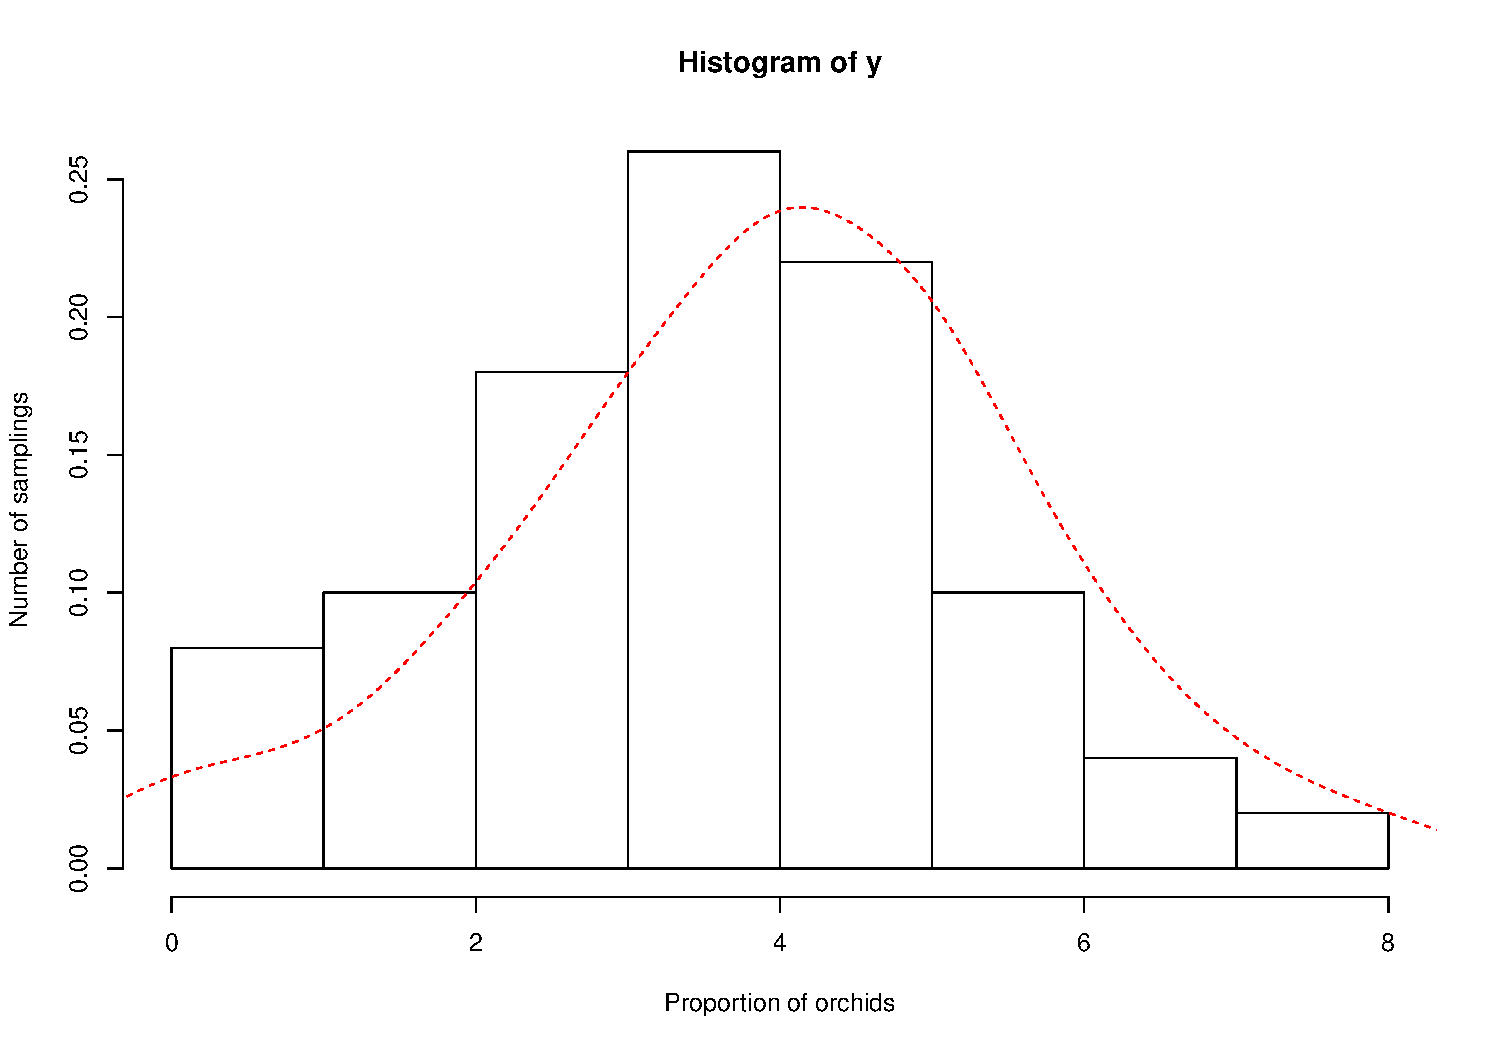
\includegraphics{IntroLM_files/figure-beamer/unnamed-chunk-2-1.pdf}
\column{0.5\textwidth} \includegraphics{grassland.jpeg} \columnsend
\end{frame}

\begin{frame}[fragile]{The orchids example}
\protect\hypertarget{the-orchids-example-1}{}
\begin{codebox}

\begin{Shaded}
\begin{Highlighting}[]
\FunctionTok{set.seed}\NormalTok{(}\DecValTok{12345}\NormalTok{) }\CommentTok{\# For reproducibility}
\NormalTok{n.times }\OtherTok{\textless{}{-}} \DecValTok{100}\NormalTok{;n.picks}\OtherTok{=}\DecValTok{1}\NormalTok{;p.orchid }\OtherTok{\textless{}{-}} \FloatTok{0.4}
\NormalTok{y }\OtherTok{\textless{}{-}} \FunctionTok{rbinom}\NormalTok{(n.times, }\AttributeTok{size =}\NormalTok{ n.picks, }\AttributeTok{prob =}\NormalTok{ p.orchid) }
\end{Highlighting}
\end{Shaded}

\end{codebox}

\columnsbegin
\column{0.5\textwidth}

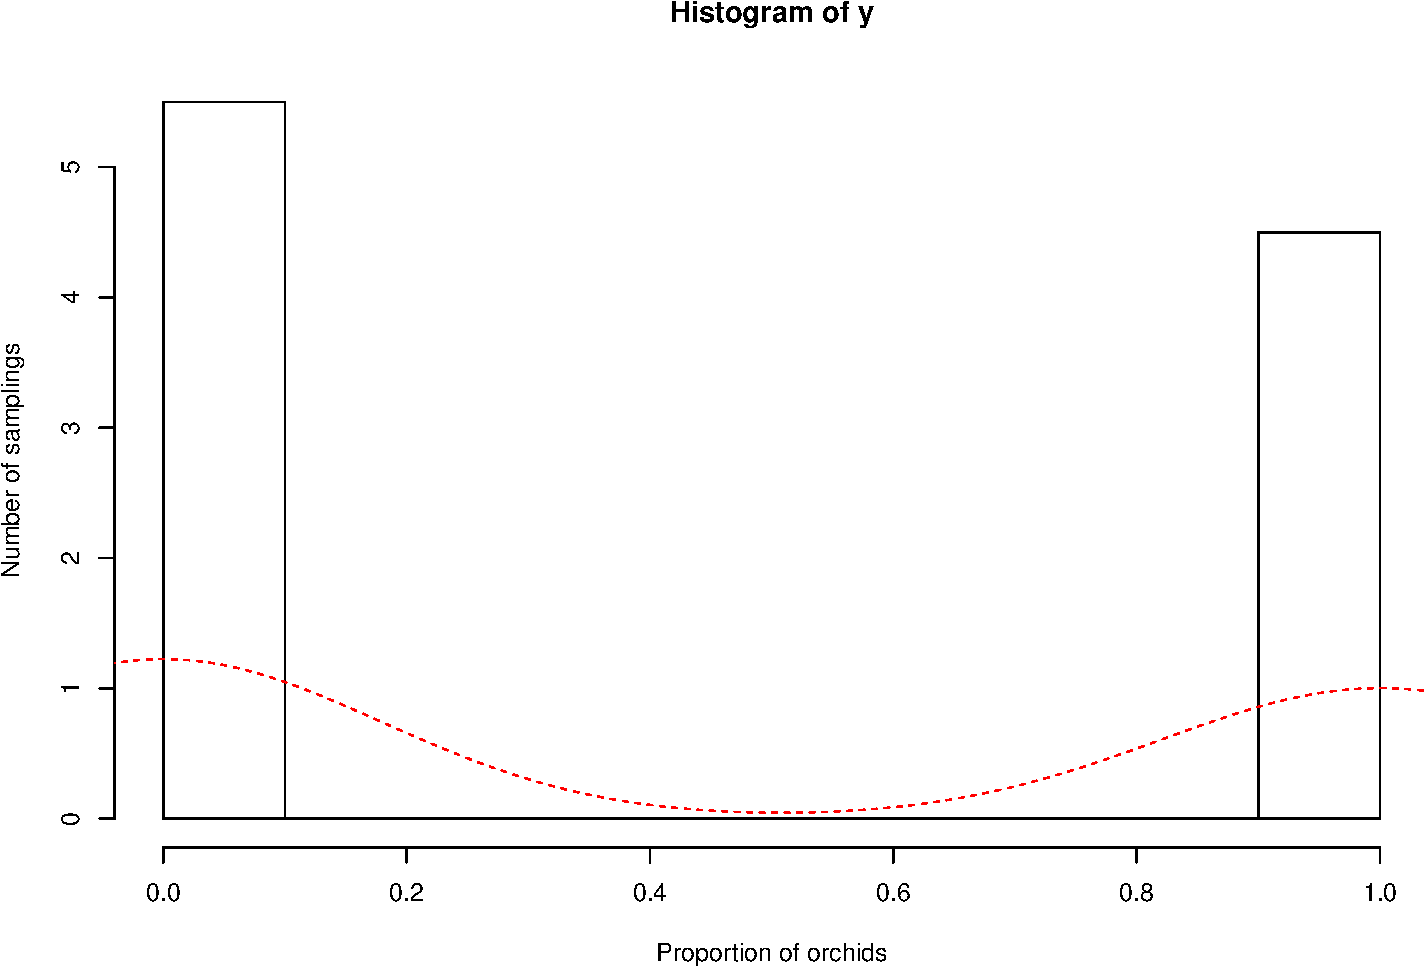
\includegraphics{IntroLM_files/figure-beamer/unnamed-chunk-4-1.pdf}
\column{0.5\textwidth} \includegraphics{grassland.jpeg} \columnsend
\end{frame}

\begin{frame}{The orchids example}
\protect\hypertarget{the-orchids-example-2}{}
The Binomial distribution is approximately normal for large
\(n_{picks}\) and \(\pi\) away from 0 and 1
\end{frame}

\begin{frame}{Normality}
\protect\hypertarget{normality}{}
\columnsbegin
\column{0.5\textwidth}

\textbf{Real ecological observations are rarely normally distributed.}\newline
But it is a nice starting point when learning GLMs.\newline We can use
it (e.g.,) when the mean is far enough from zero. \column{0.5\textwidth}
\centering 
\includegraphics{normal.jpeg} \columnsend
\end{frame}

\hypertarget{mathcalnmusigma2}{%
\section{\texorpdfstring{\(\mathcal{N}(\mu,\sigma^2)\)}{\textbackslash mathcal\{N\}(\textbackslash mu,\textbackslash sigma\^{}2)}}\label{mathcalnmusigma2}}

\begin{frame}{The normal distribution}
\protect\hypertarget{the-normal-distribution}{}
\begin{equation}
f(y_i;\mu, \sigma) = \frac{1}{\sigma\sqrt{2\pi}}\exp\biggl\{\frac{(y_i-\mu)^2}{2\sigma^2}\biggr\}
\end{equation}
\end{frame}

\begin{frame}{The normal distribution (2)}
\protect\hypertarget{the-normal-distribution-2}{}
Likelihood: \begin{equation}
f(y_i;\mu, \sigma) = \frac{1}{\sigma\sqrt{2\pi}}\exp\biggl\{\frac{(y_i-\mu)^2}{2\sigma^2}\biggr\}
\end{equation}

log-Likelihood: \begin{equation}
\log\{f(y_i;\mu, \sigma)\} = -\frac{1}{2}\log(\sigma^22\pi) -\frac{(y_i-\mu)^2}{2\sigma^2}
\end{equation} Two parameters: \(\mu\) and \(\sigma\)

\begin{itemize}
\tightlist
\item
  \(\mu\) is the mean; the middle of the distribution
\item
  \(\sigma\) is the standard deviation; it controls the width
\end{itemize}

Not only used for data, also the basis of many statistics (e.g.,
asymptotic sampling distributions)
\end{frame}

\begin{frame}{Estimating \(\mu\)}
\protect\hypertarget{estimating-mu}{}
Same process as before: calculate gradient and find estimator

\begin{equation}
\frac{\partial\log\{\mathcal{L}(\textbf{y};\hat{\mu},\sigma)\}}{\partial\mu} = \frac{1}{2\sigma^2}\biggl(2\sum \limits^n_{i=1}y_i-2n\mu\biggl)
\end{equation}

Giving..

\begin{equation}
\hat{\mu} = \frac{1}{n}\sum \limits^n_{i=1}y_i
\end{equation}

It is a linear function of \(y_i\) so is normally distributed.
\end{frame}

\begin{frame}{Estimating \(\sigma^2\)}
\protect\hypertarget{estimating-sigma2}{}
Same process as before. MLE is biased so gets a small correction.

\begin{equation}
\hat{\sigma}^2 = \frac{1}{n-1}\sum \limits^n_{i=1}(y_i-\hat{\mu})^2
\end{equation}

Is it a quadratic function of \(y_i\) so is \(\chi^2\)-distributed.
\end{frame}

\begin{frame}{Uncertainty of \(\hat{\mu}\)}
\protect\hypertarget{uncertainty-of-hatmu}{}
\begin{equation}
\begin{aligned}
\text{var}(\hat{\mu}) &= \mathams{E}(\hat{\mu}^2)-\mathams{E}(\hat{\mu})\mathams{E}(\hat{\mu})\\
&= \frac{1}{n^2}\sum\limits^n_{i=1}\mathams{E}(y_i^2)-\mathams{E}(\hat{\mu})\mathams{E}(\hat{\mu})\\
&= \frac{1}{n}\sigma^2
\end{aligned}
\end{equation}

\begin{itemize}
\tightlist
\item
  Depends on \(n\) (small \(n\), large uncertainty)
\item
  Depends on \(\sigma^2\)
\item
  Which is estimated by \(\hat{\sigma}^2\)
\item
  But that estimate also has uncertainty
\end{itemize}

So, we use the \(t\)-distribution to represent that additional
uncertainty.
\end{frame}

\begin{frame}{The t-distribution}
\protect\hypertarget{the-t-distribution}{}
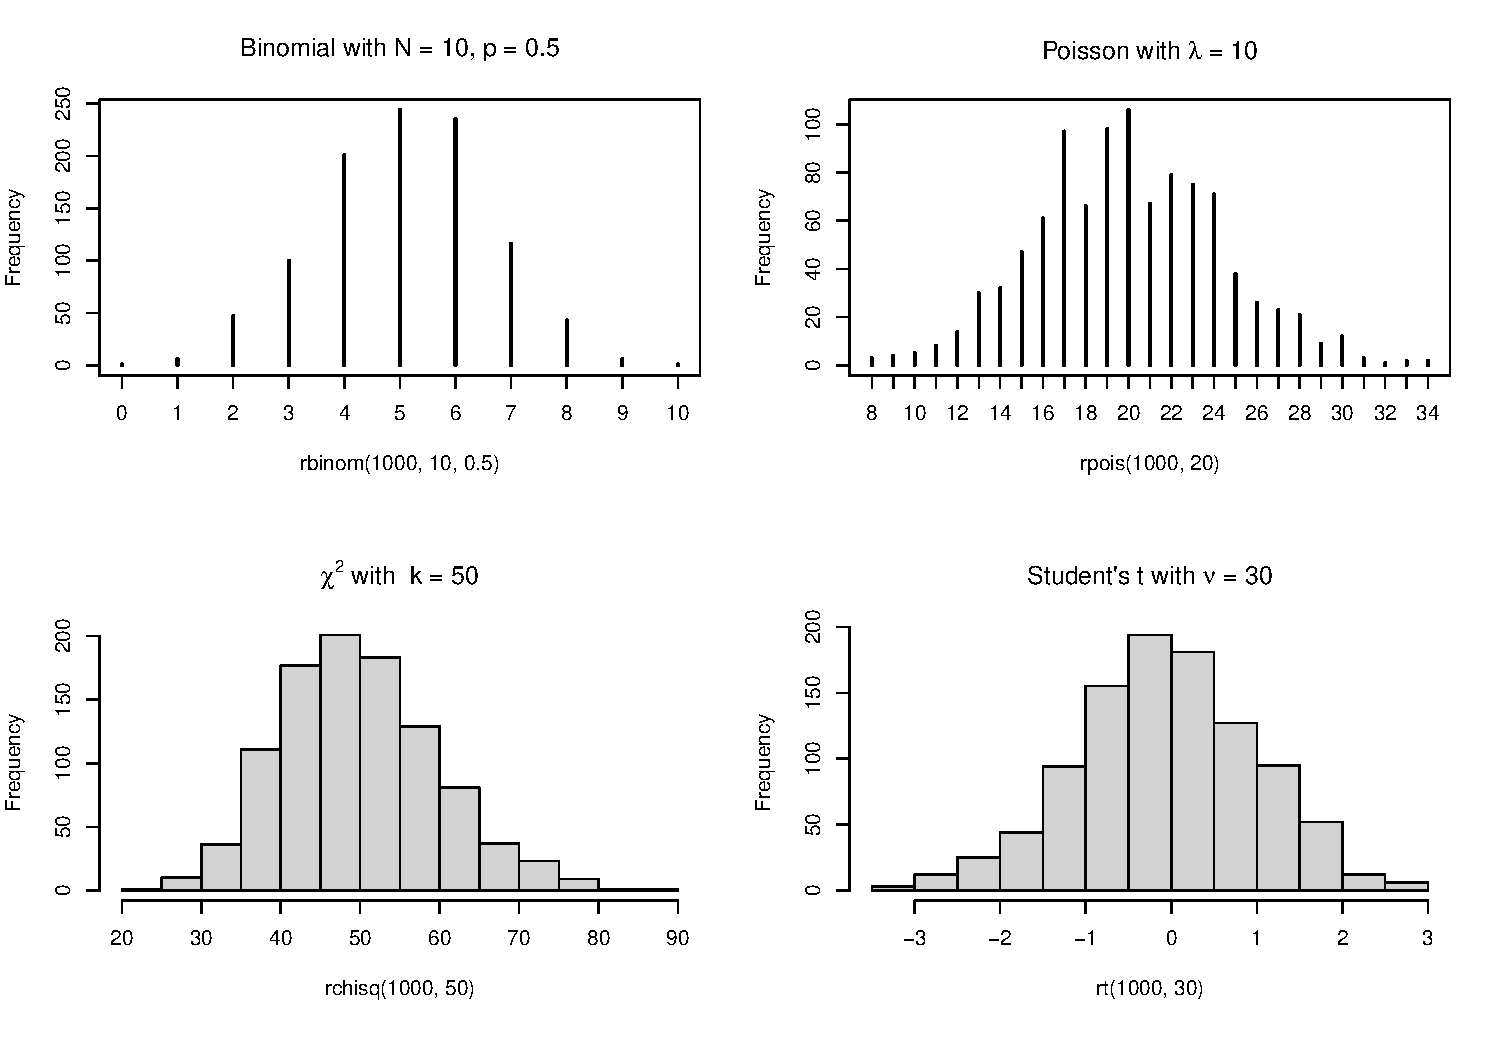
\includegraphics{IntroLM_files/figure-beamer/unnamed-chunk-5-1.pdf}
\end{frame}

\begin{frame}[fragile]{The t-test}
\protect\hypertarget{the-t-test}{}
\begin{itemize}
\tightlist
\item
  The t-test is type of linear regression
\item
  With one covariate and two groups
\end{itemize}

\tiny

\begin{codebox}

\begin{Shaded}
\begin{Highlighting}[]
\FunctionTok{set.seed}\NormalTok{(}\DecValTok{12345}\NormalTok{)}
\NormalTok{y }\OtherTok{\textless{}{-}} \FunctionTok{rnorm}\NormalTok{(}\DecValTok{10}\NormalTok{)}
\NormalTok{x }\OtherTok{\textless{}{-}} \FunctionTok{rnorm}\NormalTok{(}\DecValTok{10}\NormalTok{, }\AttributeTok{mean =} \DecValTok{2}\NormalTok{)}
\FunctionTok{t.test}\NormalTok{(x, y)}
\end{Highlighting}
\end{Shaded}

\end{codebox}

\begin{codebox}

\begin{verbatim}
## 
##  Welch Two Sample t-test
## 
## data:  x and y
## t = 6.5336, df = 17.979, p-value = 3.872e-06
## alternative hypothesis: true difference in means is not equal to 0
## 95 percent confidence interval:
##  1.641042 3.196802
## sample estimates:
##  mean of x  mean of y 
##  2.2859778 -0.1329441
\end{verbatim}

\end{codebox}

\normalsize
\end{frame}

\begin{frame}{t-test visualized}
\protect\hypertarget{t-test-visualized}{}
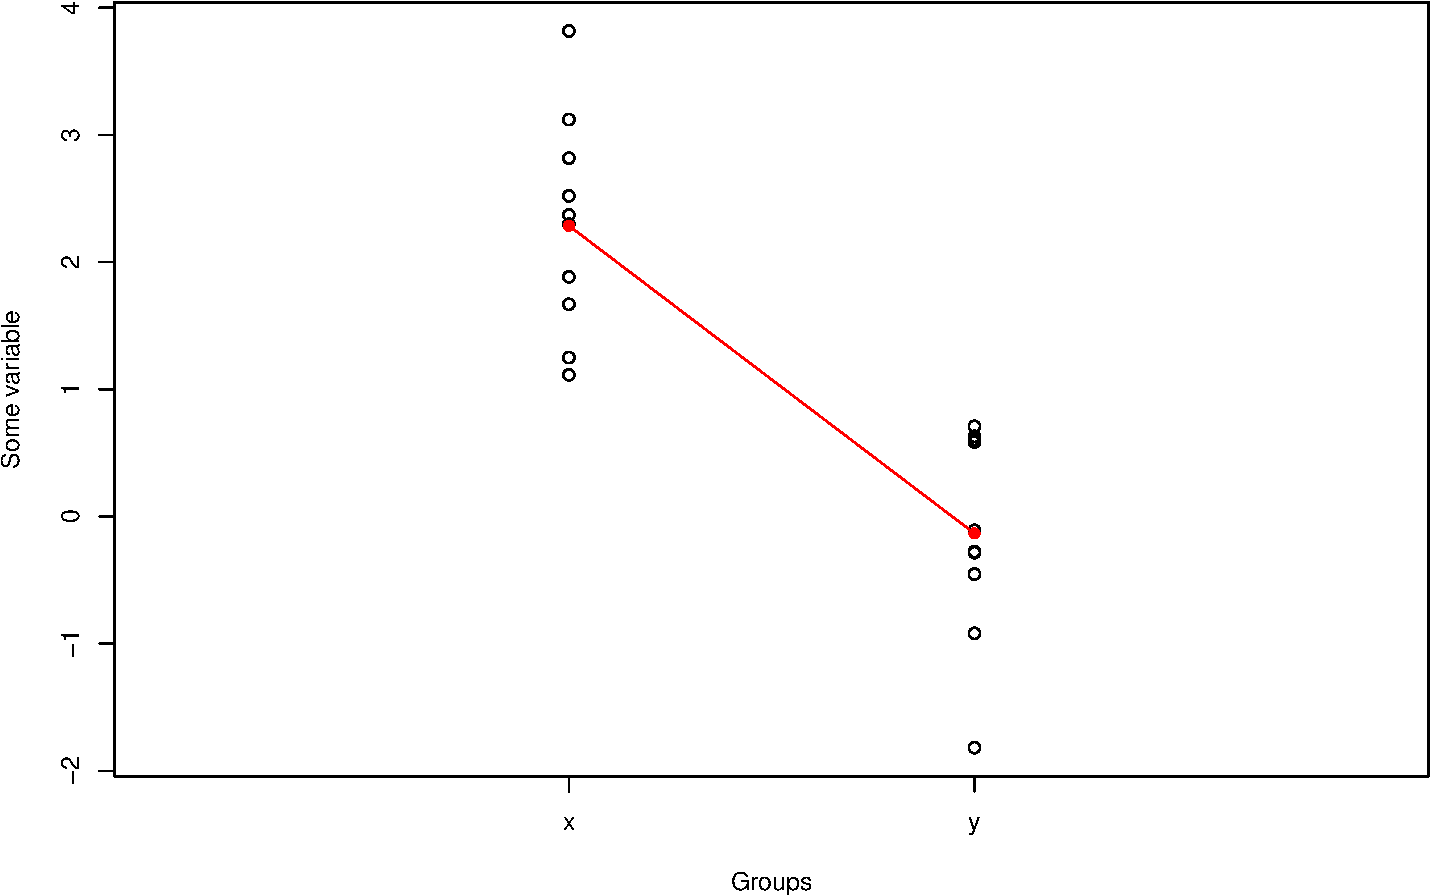
\includegraphics{IntroLM_files/figure-beamer/unnamed-chunk-7-1.pdf}
\end{frame}

\hypertarget{simple-linear-regression}{%
\section{Simple linear regression}\label{simple-linear-regression}}

\begin{frame}[fragile]{t-test as linear regression}
\protect\hypertarget{t-test-as-linear-regression}{}
\begin{codebox}

\begin{Shaded}
\begin{Highlighting}[]
\NormalTok{data }\OtherTok{\textless{}{-}} \FunctionTok{data.frame}\NormalTok{(}\AttributeTok{y =} \FunctionTok{c}\NormalTok{(x, y), }
                   \AttributeTok{var =} \FunctionTok{c}\NormalTok{(}\FunctionTok{rep}\NormalTok{(}\FunctionTok{c}\NormalTok{(}\StringTok{"x"}\NormalTok{,}\StringTok{"y"}\NormalTok{),}\AttributeTok{each=}\DecValTok{10}\NormalTok{)))}
\FunctionTok{lm}\NormalTok{(y}\SpecialCharTok{\textasciitilde{}}\DecValTok{0}\SpecialCharTok{+}\NormalTok{var, }\AttributeTok{data =}\NormalTok{ data)}
\end{Highlighting}
\end{Shaded}

\end{codebox}

\begin{codebox}

\begin{verbatim}
## 
## Call:
## lm(formula = y ~ 0 + var, data = data)
## 
## Coefficients:
##    varx     vary  
##  2.2860  -0.1329
\end{verbatim}

\end{codebox}
\end{frame}

\begin{frame}{What is a linear regression?}
\protect\hypertarget{what-is-a-linear-regression}{}
\columnsbegin
\column{0.6\textwidth}

Models with a continuous \textbf{response variable} as a function of one
or more \textbf{explanatory variable}. Variables are connected by linear
equations.

\begin{itemize}
\tightlist
\item
  \(y_i\): the \textbf{response variable}, can only be numerical
\item
  \(x_i\): the \textbf{explanatory variable}, can be categorical (0,1)
  or numerical
\end{itemize}

\column{0.4\textwidth}


\includegraphics{xy.png}

\columnsend

\begin{equation}
y_i = \textcolor{red}{\alpha + x_i\beta} + \textcolor{blue}{\epsilon_i}\sim \mathcal{N}(0,\sigma^2)
\end{equation}
\end{frame}

\begin{frame}{Synonyms}
\protect\hypertarget{synonyms}{}
\begin{itemize}
\tightlist
\item
  Covariate
\item
  Predictor (variable)
\item
  Explanatory variable
\item
  Independent variable
\end{itemize}

They all refer to \(x_i\).
\end{frame}

\begin{frame}{What is the goal of regression?}
\protect\hypertarget{what-is-the-goal-of-regression}{}
We measure data \(y_i\) and want to infer its with \(x_i\)

Steps:

\begin{enumerate}
[1)]
\tightlist
\item
  We decide on a model
\item
  We estimate the parameters
\item
  We check if it is a valid and good model
\item
  We draw our conclusion (with uncertainty)
\end{enumerate}
\end{frame}

\begin{frame}{Examples of linear models: categorical \(x_i\)}
\protect\hypertarget{examples-of-linear-models-categorical-x_i}{}
\columnsbegin
\column{0.4\textwidth}

\[
\mu_i =
  \begin{cases}
    \beta_0       & \quad \text{if } X_i =0 \\
    \beta_1      & \quad \text{if } X_i =1  
  \end{cases}
\] \[
\mu_i =
  \begin{cases}
    \alpha       & \quad \text{if } X_i =0 \\
    \alpha + \beta       & \quad \text{if } X_i =1  
  \end{cases}
\] \column{0.6\textwidth}

\(y_i = (1-x_i)\beta_0 + x_i\beta_1 + \epsilon_i\sim \mathcal{N}(0,\sigma^2)\)

\vspace{2\baselineskip}

\(y_i = \alpha+ x_i\beta_1 + \epsilon_i\sim \mathcal{N}(0,\sigma^2)\)

\columnsend
\end{frame}

\begin{frame}{Examples of linear models: categorical \(x_i\)}
\protect\hypertarget{examples-of-linear-models-categorical-x_i-1}{}
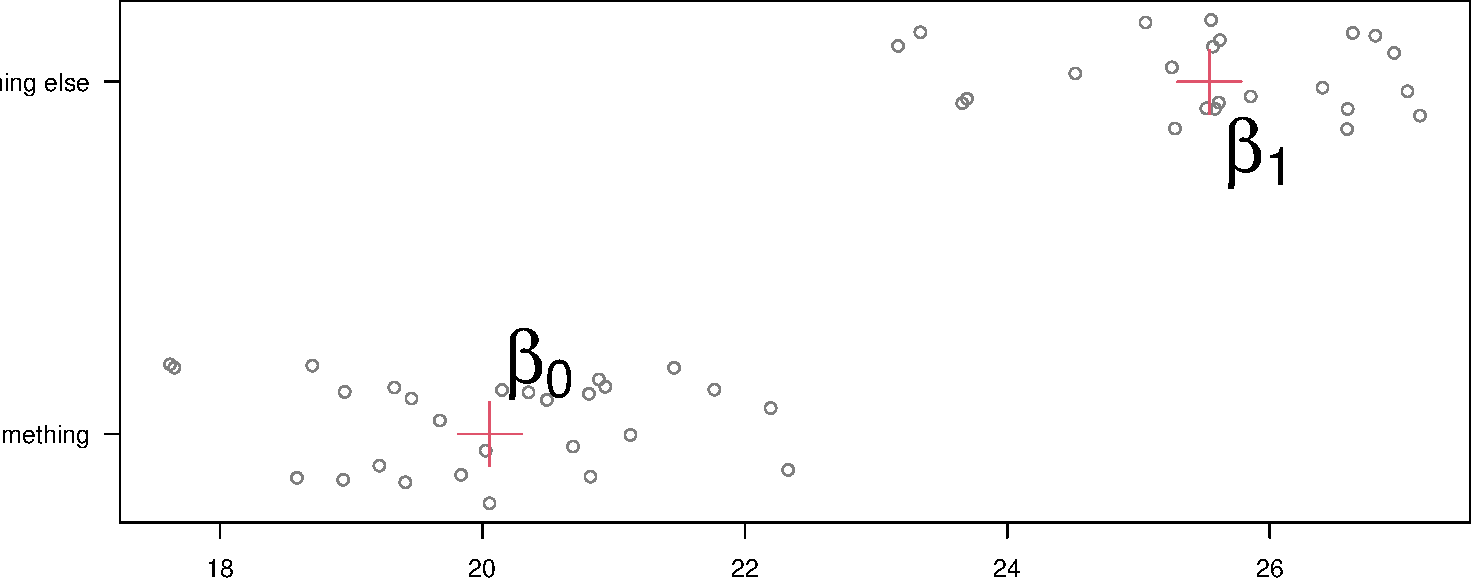
\includegraphics{IntroLM_files/figure-beamer/unnamed-chunk-9-1.pdf}

\begin{itemize}
\tightlist
\item
  \(\beta_0\) is the group 1 mean
\item
  \(\beta_1\) is the group 2 mean
\end{itemize}
\end{frame}

\begin{frame}{Examples of linear models: categorical \(x_i\)}
\protect\hypertarget{examples-of-linear-models-categorical-x_i-2}{}
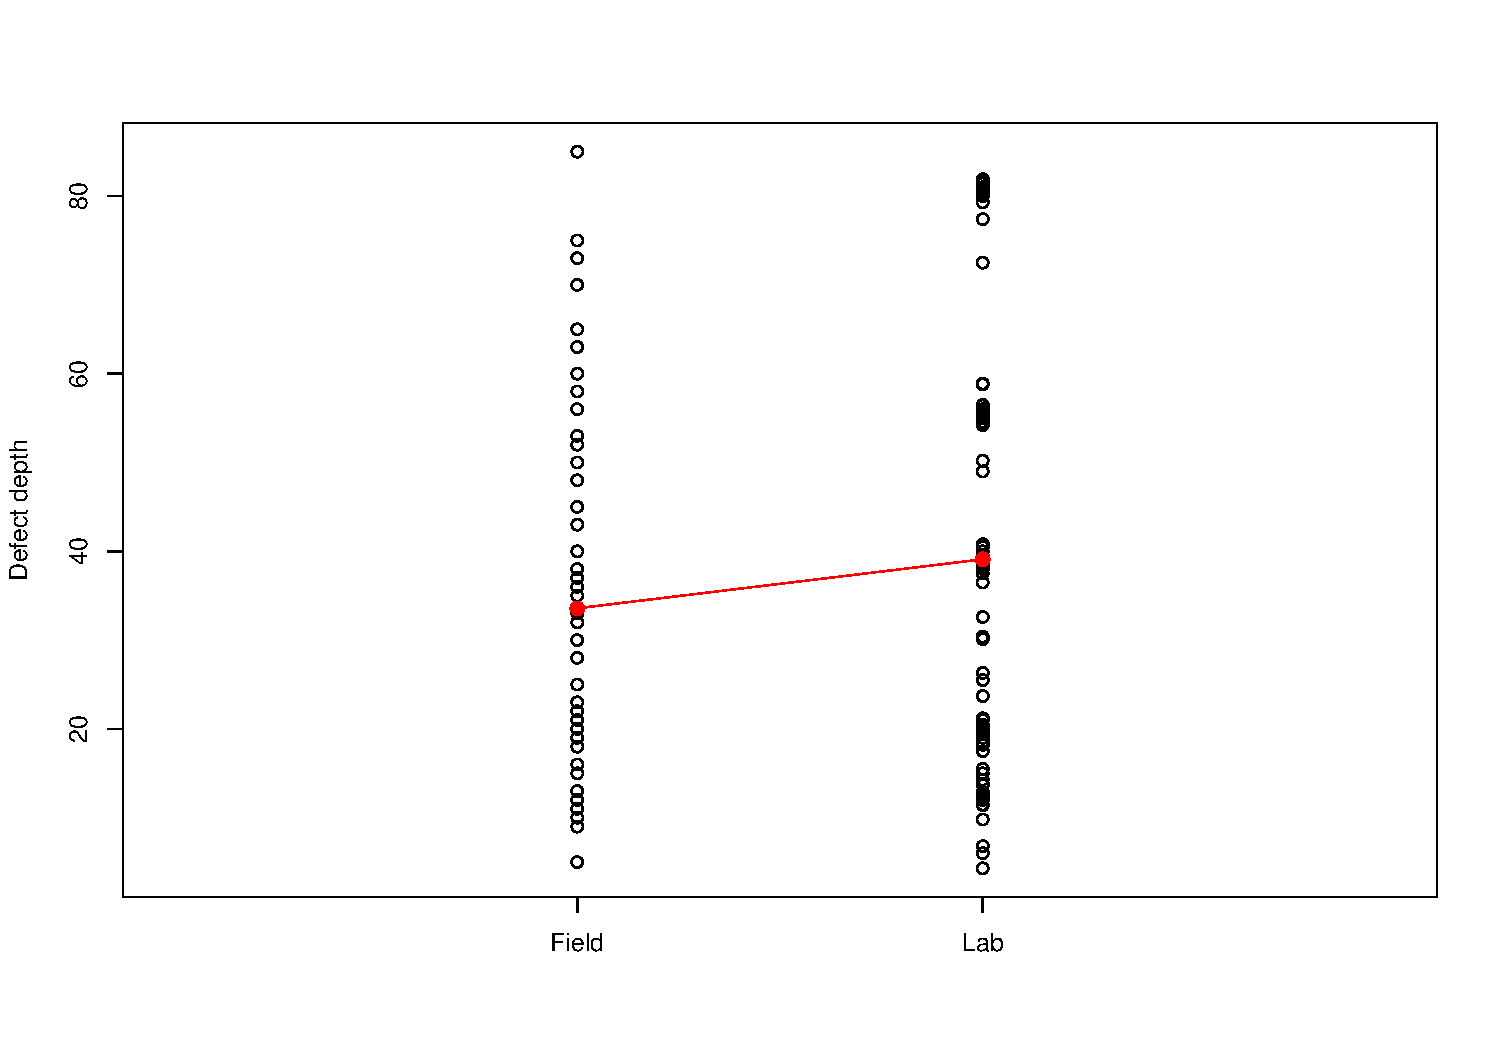
\includegraphics{IntroLM_files/figure-beamer/unnamed-chunk-10-1.pdf}

\begin{itemize}
\tightlist
\item
  \(\alpha\) is the mean of the first group
\item
  \(\beta\) is the deviation from the mean of the first group
\end{itemize}
\end{frame}

\begin{frame}{Examples of linear models: continuous \(x_i\)}
\protect\hypertarget{examples-of-linear-models-continuous-x_i}{}
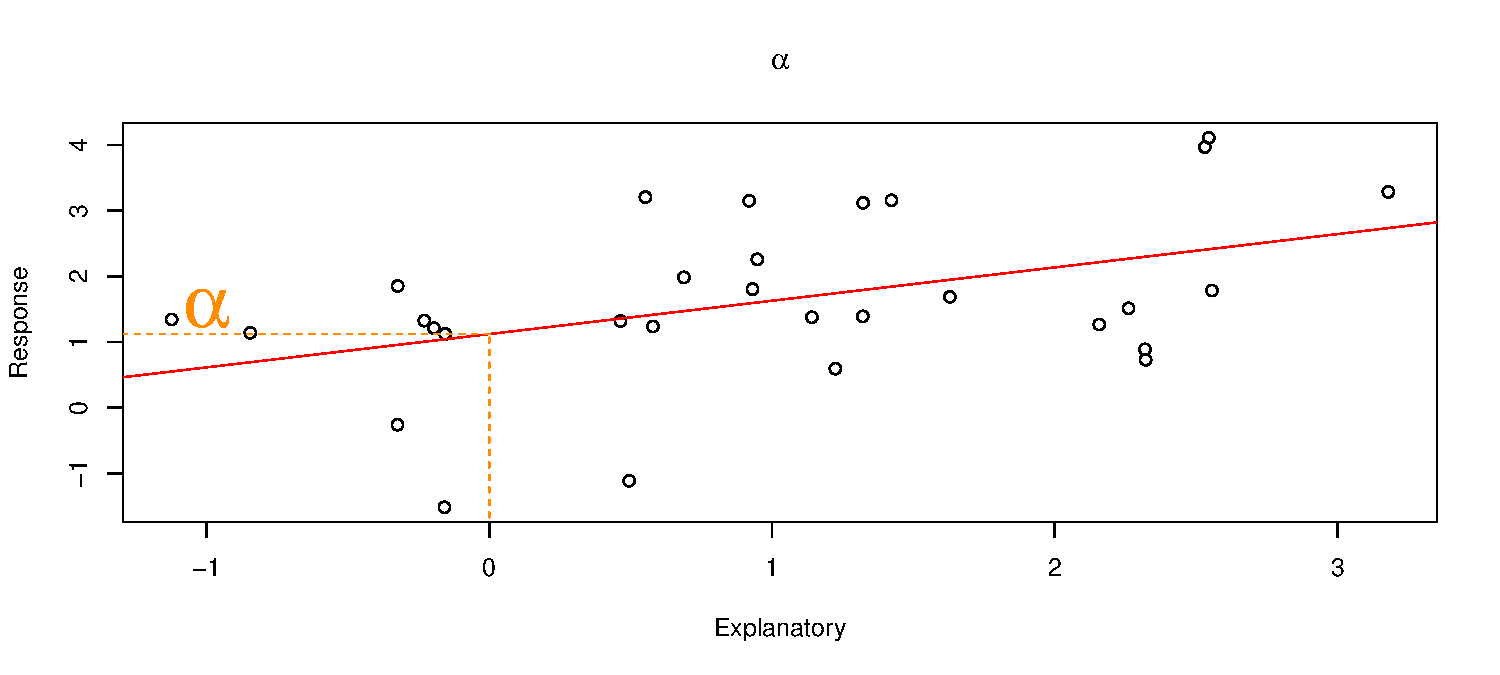
\includegraphics{IntroLM_files/figure-beamer/reg-1.pdf}

\(y_i = \textcolor{darkorange}{\alpha} + x_i\beta + \epsilon_i\sim \mathcal{N}(0,\sigma^2)\)

\begin{itemize}
\tightlist
\item
  \(\textcolor{darkorange}{\alpha}\): the intercept is the value of
  \(y_i\) where \(x_i = 0\)
\end{itemize}
\end{frame}

\begin{frame}{Examples of linear models: continuous \(x_i\)}
\protect\hypertarget{examples-of-linear-models-continuous-x_i-1}{}
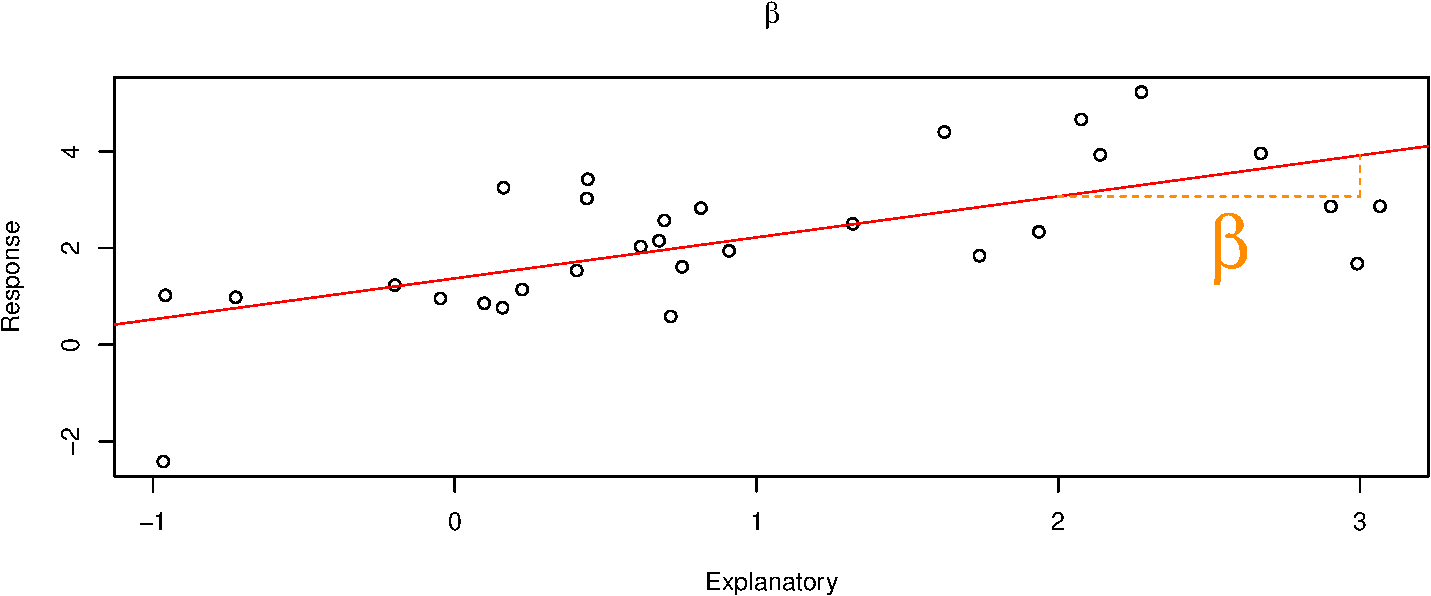
\includegraphics{IntroLM_files/figure-beamer/reg2-1.pdf}

\(y_i = \alpha + x_i\textcolor{darkorange}{\beta} + \epsilon_i\sim \mathcal{N}(0,\sigma^2)\)

\begin{itemize}
\tightlist
\item
  \(\alpha\): the intercept is the value of \(y_i\) where \(x_i = 0\)
\item
  \(\textcolor{darkorange}{\beta}\): the slope is the change in \(y_i\)
  for a unit increase in \(x_i\)
\end{itemize}
\end{frame}

\begin{frame}{What is the best line?}
\protect\hypertarget{what-is-the-best-line}{}
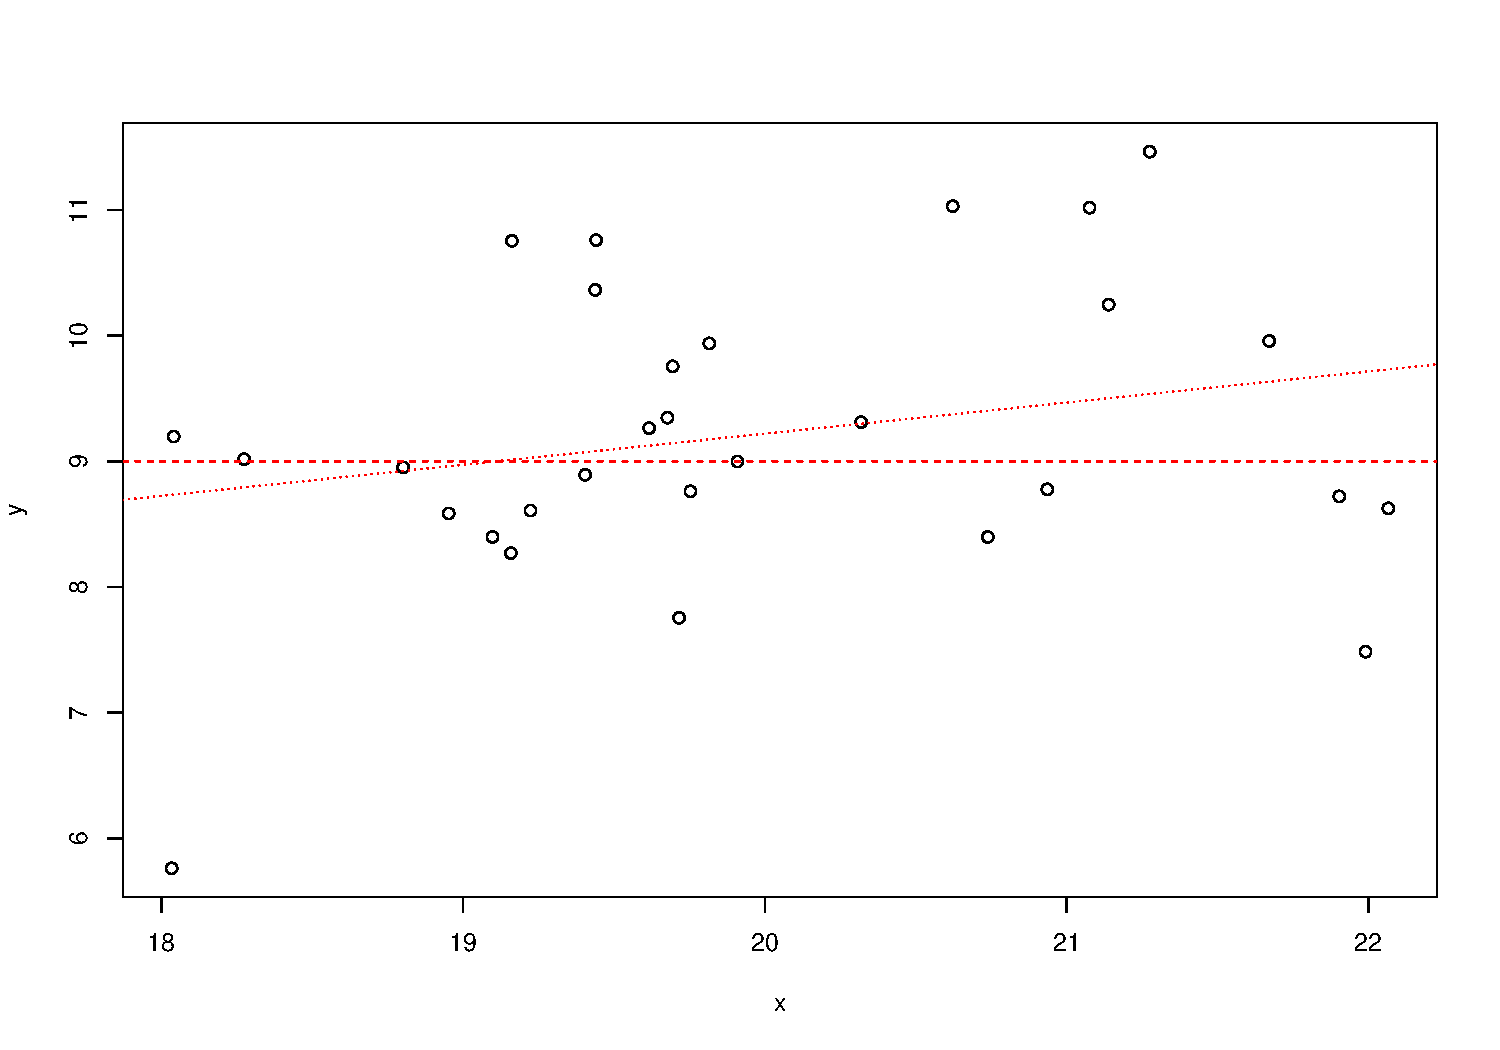
\includegraphics{IntroLM_files/figure-beamer/norm2-1.pdf}
\end{frame}

\begin{frame}{How good is the line?}
\protect\hypertarget{how-good-is-the-line}{}
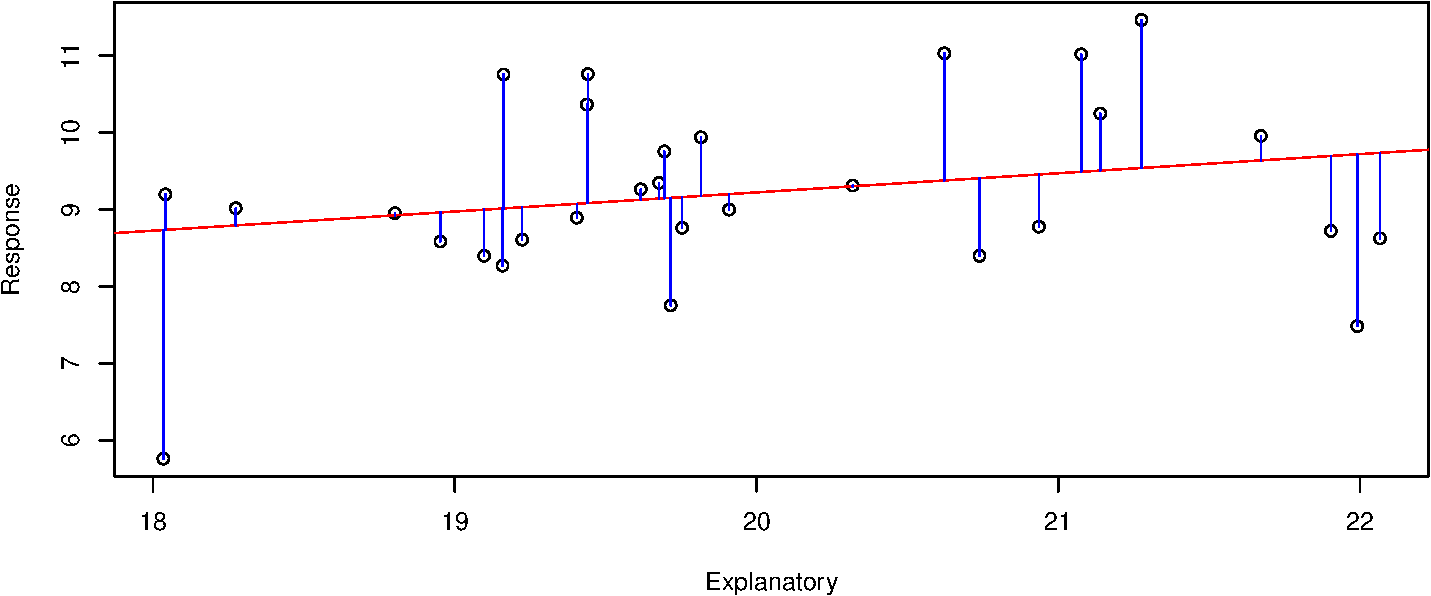
\includegraphics{IntroLM_files/figure-beamer/norm-1.pdf}

Distance from model (line) to data: ``error''
\(\textcolor{blue}{\epsilon_i}\)
\end{frame}

\begin{frame}{Least squares estimation}
\protect\hypertarget{least-squares-estimation}{}
Minimize the sum of squared residuals: \begin{equation}
RSS = \sum \limits^n_{i=1} \epsilon_i^2
\end{equation} which is the same to maximizing the normal likelihood!

\begin{itemize}
\tightlist
\item
  \(\hat{\alpha}= \frac{1}{N}(\sum y_i - \hat{\beta}\sum x_i)\)
\item
  \(\hat{\beta} = \frac{\sum (x_i - \sum \frac{x_i}{N})(y_i - \sum \frac{y_i}{N})}{\sum (x_i - \sum \frac{x_i}{N})^2}\)
\item
  \(\hat{\sigma^2} = \frac{1}{N-1}\sum (y_i - (\alpha+x_i\beta))^2\)
\item
  \(\hat{\mu}_i = \hat{\alpha}+x_i\hat{\beta}\)
\end{itemize}
\end{frame}

\begin{frame}{Our model}
\protect\hypertarget{our-model}{}
\begin{equation}
y_i = \alpha + \beta x_i + \epsilon_i\sim \mathcal{N}(0,\sigma^2)
\end{equation}

\begin{itemize}
\tightlist
\item
  \(y_i\): our data
\item
  \(\alpha\), \(\beta\) describe our line
\item
  \(\epsilon_i\) quantifies distance to the model
\end{itemize}
\end{frame}

\begin{frame}{Assumptions}
\protect\hypertarget{assumptions}{}
We make some critical assumptions here

\begin{enumerate}
[1)]
\tightlist
\item
  the relationship between \(y_i\) and \(x_i\)
\item
  distribution of the errors
\end{enumerate}
\end{frame}

\begin{frame}{Other assumptions for the Errors}
\protect\hypertarget{other-assumptions-for-the-errors}{}
\begin{equation}
\epsilon_i \overset{iid}{\sim} \mathcal{N}(0, \sigma^2)
\end{equation}

\begin{itemize}
\tightlist
\item
  are normally distributed
\item
  have constant variance (``Homoscedastcity'')
\item
  are independent
\item
  no outliers
\end{itemize}
\end{frame}

\begin{frame}{Assumptions for the errors}
\protect\hypertarget{assumptions-for-the-errors}{}
\textbf{all the errors together tell us how good the line is}

\begin{itemize}
\tightlist
\item
  this is the same as finding the line by maximum likelihood estimation
  \emoji{smile}
\end{itemize}

\begin{equation}
y_i \sim \mathcal{N}(\alpha+x_i\beta, \sigma^2)
\end{equation}
\end{frame}

\begin{frame}{Summary simple linear models}
\protect\hypertarget{summary-simple-linear-models}{}
\begin{itemize}
\tightlist
\item
  includes t-test, anova (analysis of variance) and regression
\item
  all use the same mathy bits (and model)
\item
  \textbf{interpretation} depends on the type of \textbf{variable}
\item
  GLMs take the same form
\end{itemize}
\end{frame}

\begin{frame}[fragile]{Summary}
\protect\hypertarget{summary}{}
\begin{itemize}
\tightlist
\item
  Normal-distribution and t-distribution
\item
  Simple linear regression: one covariate
\item
  Least squares estimation
\item
  Difference in LMs with categorical or continuous explanatory variables

  \begin{itemize}
  \tightlist
  \item
    Categorical: intercept/mean parameter
  \item
    Continuous: slope parameter
  \end{itemize}
\item
  Fortunately we have the \texttt{lm()} function in R!
\item
  More on assumptions checking tomorrow
\end{itemize}
\end{frame}

\begin{frame}{Summary (2)}
\protect\hypertarget{summary-2}{}
t-test: linear model with categorical covariate of two groups ANOVA:
linear model with categorical covariate of multiple groups ANCOVA:
linear model with categorical and continuous covariate (interaction)
\end{frame}

\end{document}
